% Created by tikzDevice version 0.12 on 2019-03-22 15:25:49
% !TEX encoding = UTF-8 Unicode
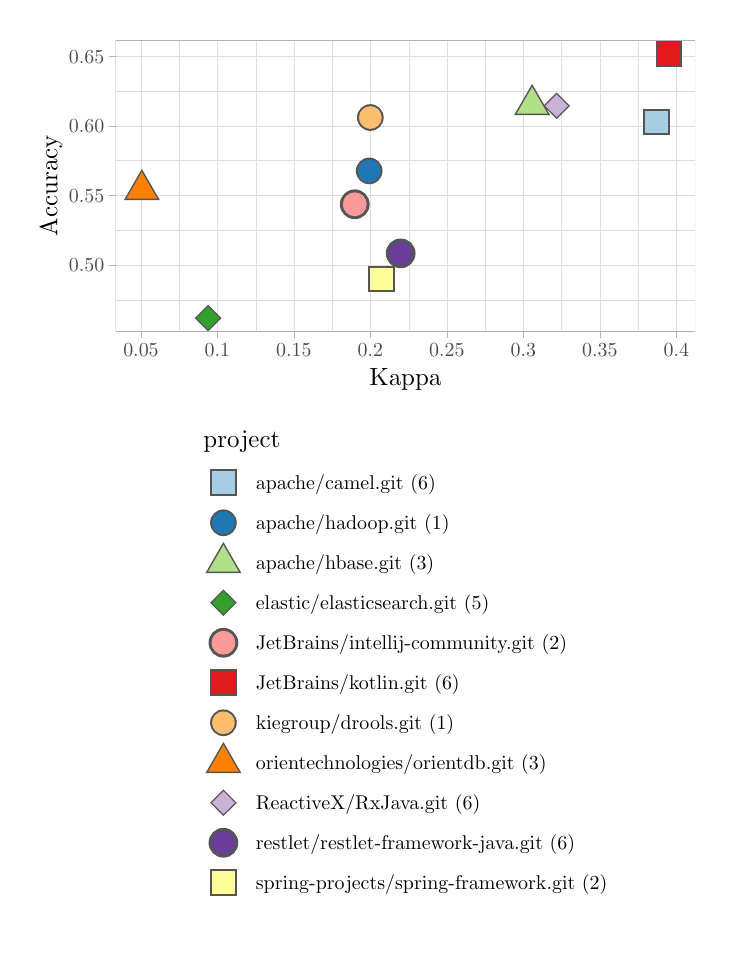
\begin{tikzpicture}[x=1pt,y=1pt]
\definecolor{fillColor}{RGB}{255,255,255}
\path[use as bounding box,fill=fillColor,fill opacity=0.00] (0,0) rectangle (245.72,325.21);
\begin{scope}
\path[clip] (  0.00,  0.00) rectangle (245.72,325.21);
\definecolor{drawColor}{RGB}{255,255,255}
\definecolor{fillColor}{RGB}{255,255,255}

\path[draw=drawColor,line width= 0.5pt,line join=round,line cap=round,fill=fillColor] (  0.00,  0.00) rectangle (245.72,325.21);
\end{scope}
\begin{scope}
\path[clip] ( 31.74,215.48) rectangle (241.22,320.71);
\definecolor{fillColor}{RGB}{255,255,255}

\path[fill=fillColor] ( 31.74,215.48) rectangle (241.22,320.71);
\definecolor{drawColor}{gray}{0.87}

\path[draw=drawColor,line width= 0.1pt,line join=round] ( 31.74,226.85) --
	(241.22,226.85);

\path[draw=drawColor,line width= 0.1pt,line join=round] ( 31.74,252.01) --
	(241.22,252.01);

\path[draw=drawColor,line width= 0.1pt,line join=round] ( 31.74,277.17) --
	(241.22,277.17);

\path[draw=drawColor,line width= 0.1pt,line join=round] ( 31.74,302.33) --
	(241.22,302.33);

\path[draw=drawColor,line width= 0.1pt,line join=round] ( 54.75,215.48) --
	( 54.75,320.71);

\path[draw=drawColor,line width= 0.1pt,line join=round] ( 82.39,215.48) --
	( 82.39,320.71);

\path[draw=drawColor,line width= 0.1pt,line join=round] (110.02,215.48) --
	(110.02,320.71);

\path[draw=drawColor,line width= 0.1pt,line join=round] (137.66,215.48) --
	(137.66,320.71);

\path[draw=drawColor,line width= 0.1pt,line join=round] (165.29,215.48) --
	(165.29,320.71);

\path[draw=drawColor,line width= 0.1pt,line join=round] (192.93,215.48) --
	(192.93,320.71);

\path[draw=drawColor,line width= 0.1pt,line join=round] (220.57,215.48) --
	(220.57,320.71);

\path[draw=drawColor,line width= 0.2pt,line join=round] ( 31.74,239.43) --
	(241.22,239.43);

\path[draw=drawColor,line width= 0.2pt,line join=round] ( 31.74,264.59) --
	(241.22,264.59);

\path[draw=drawColor,line width= 0.2pt,line join=round] ( 31.74,289.75) --
	(241.22,289.75);

\path[draw=drawColor,line width= 0.2pt,line join=round] ( 31.74,314.92) --
	(241.22,314.92);

\path[draw=drawColor,line width= 0.2pt,line join=round] ( 40.94,215.48) --
	( 40.94,320.71);

\path[draw=drawColor,line width= 0.2pt,line join=round] ( 68.57,215.48) --
	( 68.57,320.71);

\path[draw=drawColor,line width= 0.2pt,line join=round] ( 96.21,215.48) --
	( 96.21,320.71);

\path[draw=drawColor,line width= 0.2pt,line join=round] (123.84,215.48) --
	(123.84,320.71);

\path[draw=drawColor,line width= 0.2pt,line join=round] (151.48,215.48) --
	(151.48,320.71);

\path[draw=drawColor,line width= 0.2pt,line join=round] (179.11,215.48) --
	(179.11,320.71);

\path[draw=drawColor,line width= 0.2pt,line join=round] (206.75,215.48) --
	(206.75,320.71);

\path[draw=drawColor,line width= 0.2pt,line join=round] (234.38,215.48) --
	(234.38,320.71);
\definecolor{fillColor}{RGB}{85,85,85}

\path[fill=fillColor] (222.45,286.31) --
	(232.08,286.31) --
	(232.08,295.94) --
	(222.45,295.94) --
	cycle;
\definecolor{drawColor}{RGB}{85,85,85}

\path[draw=drawColor,line width= 1.1pt,line join=round,line cap=round,fill=fillColor] (134.78,243.65) circle (  4.82);

\path[fill=fillColor] (226.88,311.12) --
	(236.51,311.12) --
	(236.51,320.75) --
	(226.88,320.75) --
	cycle;

\path[fill=fillColor] (186.33,296.97) --
	(191.15,301.79) --
	(195.96,296.97) --
	(191.15,292.16) --
	cycle;

\path[fill=fillColor] ( 60.38,220.26) --
	( 65.19,225.08) --
	( 70.01,220.26) --
	( 65.19,215.45) --
	cycle;

\path[fill=fillColor] (182.28,304.87) --
	(188.77,293.63) --
	(175.79,293.63) --
	cycle;

\path[fill=fillColor] ( 41.26,274.14) --
	( 47.75,262.91) --
	( 34.78,262.91) --
	cycle;

\path[draw=drawColor,line width= 1.1pt,line join=round,line cap=round,fill=fillColor] (118.19,261.39) circle (  4.82);

\path[fill=fillColor] (122.94,229.58) --
	(132.57,229.58) --
	(132.57,239.21) --
	(122.94,239.21) --
	cycle;

\path[fill=fillColor] (123.41,273.44) circle (  4.82);

\path[fill=fillColor] (123.81,292.74) circle (  4.82);
\definecolor{fillColor}{RGB}{166,206,227}

\path[fill=fillColor] (223.16,287.02) --
	(231.37,287.02) --
	(231.37,295.23) --
	(223.16,295.23) --
	cycle;
\definecolor{drawColor}{RGB}{106,61,154}
\definecolor{fillColor}{RGB}{106,61,154}

\path[draw=drawColor,line width= 0.4pt,line join=round,line cap=round,fill=fillColor] (134.78,243.65) circle (  4.10);
\definecolor{fillColor}{RGB}{227,26,28}

\path[fill=fillColor] (227.59,311.83) --
	(235.80,311.83) --
	(235.80,320.04) --
	(227.59,320.04) --
	cycle;
\definecolor{fillColor}{RGB}{202,178,214}

\path[fill=fillColor] (187.04,296.97) --
	(191.15,301.08) --
	(195.25,296.97) --
	(191.15,292.87) --
	cycle;
\definecolor{fillColor}{RGB}{51,160,44}

\path[fill=fillColor] ( 61.09,220.26) --
	( 65.19,224.37) --
	( 69.30,220.26) --
	( 65.19,216.16) --
	cycle;
\definecolor{fillColor}{RGB}{178,223,138}

\path[fill=fillColor] (182.28,303.76) --
	(187.81,294.19) --
	(176.75,294.19) --
	cycle;
\definecolor{fillColor}{RGB}{255,127,0}

\path[fill=fillColor] ( 41.26,273.03) --
	( 46.79,263.46) --
	( 35.73,263.46) --
	cycle;
\definecolor{drawColor}{RGB}{251,154,153}
\definecolor{fillColor}{RGB}{251,154,153}

\path[draw=drawColor,line width= 0.4pt,line join=round,line cap=round,fill=fillColor] (118.19,261.39) circle (  4.10);
\definecolor{fillColor}{RGB}{255,255,153}

\path[fill=fillColor] (123.65,230.29) --
	(131.86,230.29) --
	(131.86,238.50) --
	(123.65,238.50) --
	cycle;
\definecolor{fillColor}{RGB}{31,120,180}

\path[fill=fillColor] (123.41,273.44) circle (  4.10);
\definecolor{fillColor}{RGB}{253,191,111}

\path[fill=fillColor] (123.81,292.74) circle (  4.10);
\definecolor{drawColor}{gray}{0.70}

\path[draw=drawColor,line width= 0.5pt,line join=round,line cap=round] ( 31.74,215.48) rectangle (241.22,320.71);
\end{scope}
\begin{scope}
\path[clip] (  0.00,  0.00) rectangle (245.72,325.21);
\definecolor{drawColor}{gray}{0.30}

\node[text=drawColor,anchor=base east,inner sep=0pt, outer sep=0pt, scale=  0.72] at ( 27.69,236.95) {0.50};

\node[text=drawColor,anchor=base east,inner sep=0pt, outer sep=0pt, scale=  0.72] at ( 27.69,262.11) {0.55};

\node[text=drawColor,anchor=base east,inner sep=0pt, outer sep=0pt, scale=  0.72] at ( 27.69,287.27) {0.60};

\node[text=drawColor,anchor=base east,inner sep=0pt, outer sep=0pt, scale=  0.72] at ( 27.69,312.44) {0.65};
\end{scope}
\begin{scope}
\path[clip] (  0.00,  0.00) rectangle (245.72,325.21);
\definecolor{drawColor}{gray}{0.70}

\path[draw=drawColor,line width= 0.2pt,line join=round] ( 29.49,239.43) --
	( 31.74,239.43);

\path[draw=drawColor,line width= 0.2pt,line join=round] ( 29.49,264.59) --
	( 31.74,264.59);

\path[draw=drawColor,line width= 0.2pt,line join=round] ( 29.49,289.75) --
	( 31.74,289.75);

\path[draw=drawColor,line width= 0.2pt,line join=round] ( 29.49,314.92) --
	( 31.74,314.92);
\end{scope}
\begin{scope}
\path[clip] (  0.00,  0.00) rectangle (245.72,325.21);
\definecolor{drawColor}{gray}{0.70}

\path[draw=drawColor,line width= 0.2pt,line join=round] ( 40.94,213.23) --
	( 40.94,215.48);

\path[draw=drawColor,line width= 0.2pt,line join=round] ( 68.57,213.23) --
	( 68.57,215.48);

\path[draw=drawColor,line width= 0.2pt,line join=round] ( 96.21,213.23) --
	( 96.21,215.48);

\path[draw=drawColor,line width= 0.2pt,line join=round] (123.84,213.23) --
	(123.84,215.48);

\path[draw=drawColor,line width= 0.2pt,line join=round] (151.48,213.23) --
	(151.48,215.48);

\path[draw=drawColor,line width= 0.2pt,line join=round] (179.11,213.23) --
	(179.11,215.48);

\path[draw=drawColor,line width= 0.2pt,line join=round] (206.75,213.23) --
	(206.75,215.48);

\path[draw=drawColor,line width= 0.2pt,line join=round] (234.38,213.23) --
	(234.38,215.48);
\end{scope}
\begin{scope}
\path[clip] (  0.00,  0.00) rectangle (245.72,325.21);
\definecolor{drawColor}{gray}{0.30}

\node[text=drawColor,anchor=base,inner sep=0pt, outer sep=0pt, scale=  0.72] at ( 40.94,206.47) {0.05};

\node[text=drawColor,anchor=base,inner sep=0pt, outer sep=0pt, scale=  0.72] at ( 68.57,206.47) {0.1};

\node[text=drawColor,anchor=base,inner sep=0pt, outer sep=0pt, scale=  0.72] at ( 96.21,206.47) {0.15};

\node[text=drawColor,anchor=base,inner sep=0pt, outer sep=0pt, scale=  0.72] at (123.84,206.47) {0.2};

\node[text=drawColor,anchor=base,inner sep=0pt, outer sep=0pt, scale=  0.72] at (151.48,206.47) {0.25};

\node[text=drawColor,anchor=base,inner sep=0pt, outer sep=0pt, scale=  0.72] at (179.11,206.47) {0.3};

\node[text=drawColor,anchor=base,inner sep=0pt, outer sep=0pt, scale=  0.72] at (206.75,206.47) {0.35};

\node[text=drawColor,anchor=base,inner sep=0pt, outer sep=0pt, scale=  0.72] at (234.38,206.47) {0.4};
\end{scope}
\begin{scope}
\path[clip] (  0.00,  0.00) rectangle (245.72,325.21);
\definecolor{drawColor}{RGB}{0,0,0}

\node[text=drawColor,anchor=base,inner sep=0pt, outer sep=0pt, scale=  0.90] at (136.48,196.08) {Kappa};
\end{scope}
\begin{scope}
\path[clip] (  0.00,  0.00) rectangle (245.72,325.21);
\definecolor{drawColor}{RGB}{0,0,0}

\node[text=drawColor,rotate= 90.00,anchor=base,inner sep=0pt, outer sep=0pt, scale=  0.90] at ( 10.70,268.10) {Accuracy};
\end{scope}
\begin{scope}
\path[clip] (  0.00,  0.00) rectangle (245.72,325.21);
\definecolor{fillColor}{RGB}{255,255,255}

\path[fill=fillColor] ( 59.01,  4.50) rectangle (213.95,185.14);
\end{scope}
\begin{scope}
\path[clip] (  0.00,  0.00) rectangle (245.72,325.21);
\definecolor{drawColor}{RGB}{0,0,0}

\node[text=drawColor,anchor=base west,inner sep=0pt, outer sep=0pt, scale=  0.90] at ( 63.51,173.47) {project};
\end{scope}
\begin{scope}
\path[clip] (  0.00,  0.00) rectangle (245.72,325.21);
\definecolor{fillColor}{RGB}{255,255,255}

\path[fill=fillColor] ( 63.51,153.54) rectangle ( 77.96,167.99);
\end{scope}
\begin{scope}
\path[clip] (  0.00,  0.00) rectangle (245.72,325.21);
\definecolor{fillColor}{RGB}{85,85,85}

\path[fill=fillColor] ( 65.92,155.95) --
	( 75.55,155.95) --
	( 75.55,165.58) --
	( 65.92,165.58) --
	cycle;
\end{scope}
\begin{scope}
\path[clip] (  0.00,  0.00) rectangle (245.72,325.21);
\definecolor{fillColor}{RGB}{166,206,227}

\path[fill=fillColor] ( 66.63,156.66) --
	( 74.84,156.66) --
	( 74.84,164.87) --
	( 66.63,164.87) --
	cycle;
\end{scope}
\begin{scope}
\path[clip] (  0.00,  0.00) rectangle (245.72,325.21);
\definecolor{fillColor}{RGB}{255,255,255}

\path[fill=fillColor] ( 63.51,139.09) rectangle ( 77.96,153.54);
\end{scope}
\begin{scope}
\path[clip] (  0.00,  0.00) rectangle (245.72,325.21);
\definecolor{fillColor}{RGB}{85,85,85}

\path[fill=fillColor] ( 70.73,146.31) circle (  4.82);
\end{scope}
\begin{scope}
\path[clip] (  0.00,  0.00) rectangle (245.72,325.21);
\definecolor{fillColor}{RGB}{31,120,180}

\path[fill=fillColor] ( 70.73,146.31) circle (  4.10);
\end{scope}
\begin{scope}
\path[clip] (  0.00,  0.00) rectangle (245.72,325.21);
\definecolor{fillColor}{RGB}{255,255,255}

\path[fill=fillColor] ( 63.51,124.63) rectangle ( 77.96,139.09);
\end{scope}
\begin{scope}
\path[clip] (  0.00,  0.00) rectangle (245.72,325.21);
\definecolor{fillColor}{RGB}{85,85,85}

\path[fill=fillColor] ( 70.73,139.35) --
	( 77.22,128.11) --
	( 64.25,128.11) --
	cycle;
\end{scope}
\begin{scope}
\path[clip] (  0.00,  0.00) rectangle (245.72,325.21);
\definecolor{fillColor}{RGB}{178,223,138}

\path[fill=fillColor] ( 70.73,138.24) --
	( 76.26,128.67) --
	( 65.21,128.67) --
	cycle;
\end{scope}
\begin{scope}
\path[clip] (  0.00,  0.00) rectangle (245.72,325.21);
\definecolor{fillColor}{RGB}{255,255,255}

\path[fill=fillColor] ( 63.51,110.18) rectangle ( 77.96,124.63);
\end{scope}
\begin{scope}
\path[clip] (  0.00,  0.00) rectangle (245.72,325.21);
\definecolor{fillColor}{RGB}{85,85,85}

\path[fill=fillColor] ( 65.92,117.41) --
	( 70.73,122.22) --
	( 75.55,117.41) --
	( 70.73,112.59) --
	cycle;
\end{scope}
\begin{scope}
\path[clip] (  0.00,  0.00) rectangle (245.72,325.21);
\definecolor{fillColor}{RGB}{51,160,44}

\path[fill=fillColor] ( 66.63,117.41) --
	( 70.73,121.51) --
	( 74.84,117.41) --
	( 70.73,113.30) --
	cycle;
\end{scope}
\begin{scope}
\path[clip] (  0.00,  0.00) rectangle (245.72,325.21);
\definecolor{fillColor}{RGB}{255,255,255}

\path[fill=fillColor] ( 63.51, 95.72) rectangle ( 77.96,110.18);
\end{scope}
\begin{scope}
\path[clip] (  0.00,  0.00) rectangle (245.72,325.21);
\definecolor{drawColor}{RGB}{85,85,85}
\definecolor{fillColor}{RGB}{85,85,85}

\path[draw=drawColor,line width= 1.1pt,line join=round,line cap=round,fill=fillColor] ( 70.73,102.95) circle (  4.82);
\end{scope}
\begin{scope}
\path[clip] (  0.00,  0.00) rectangle (245.72,325.21);
\definecolor{drawColor}{RGB}{251,154,153}
\definecolor{fillColor}{RGB}{251,154,153}

\path[draw=drawColor,line width= 0.4pt,line join=round,line cap=round,fill=fillColor] ( 70.73,102.95) circle (  4.10);
\end{scope}
\begin{scope}
\path[clip] (  0.00,  0.00) rectangle (245.72,325.21);
\definecolor{fillColor}{RGB}{255,255,255}

\path[fill=fillColor] ( 63.51, 81.27) rectangle ( 77.96, 95.72);
\end{scope}
\begin{scope}
\path[clip] (  0.00,  0.00) rectangle (245.72,325.21);
\definecolor{fillColor}{RGB}{85,85,85}

\path[fill=fillColor] ( 65.92, 83.68) --
	( 75.55, 83.68) --
	( 75.55, 93.31) --
	( 65.92, 93.31) --
	cycle;
\end{scope}
\begin{scope}
\path[clip] (  0.00,  0.00) rectangle (245.72,325.21);
\definecolor{fillColor}{RGB}{227,26,28}

\path[fill=fillColor] ( 66.63, 84.39) --
	( 74.84, 84.39) --
	( 74.84, 92.60) --
	( 66.63, 92.60) --
	cycle;
\end{scope}
\begin{scope}
\path[clip] (  0.00,  0.00) rectangle (245.72,325.21);
\definecolor{fillColor}{RGB}{255,255,255}

\path[fill=fillColor] ( 63.51, 66.82) rectangle ( 77.96, 81.27);
\end{scope}
\begin{scope}
\path[clip] (  0.00,  0.00) rectangle (245.72,325.21);
\definecolor{fillColor}{RGB}{85,85,85}

\path[fill=fillColor] ( 70.73, 74.04) circle (  4.82);
\end{scope}
\begin{scope}
\path[clip] (  0.00,  0.00) rectangle (245.72,325.21);
\definecolor{fillColor}{RGB}{253,191,111}

\path[fill=fillColor] ( 70.73, 74.04) circle (  4.10);
\end{scope}
\begin{scope}
\path[clip] (  0.00,  0.00) rectangle (245.72,325.21);
\definecolor{fillColor}{RGB}{255,255,255}

\path[fill=fillColor] ( 63.51, 52.36) rectangle ( 77.96, 66.82);
\end{scope}
\begin{scope}
\path[clip] (  0.00,  0.00) rectangle (245.72,325.21);
\definecolor{fillColor}{RGB}{85,85,85}

\path[fill=fillColor] ( 70.73, 67.08) --
	( 77.22, 55.84) --
	( 64.25, 55.84) --
	cycle;
\end{scope}
\begin{scope}
\path[clip] (  0.00,  0.00) rectangle (245.72,325.21);
\definecolor{fillColor}{RGB}{255,127,0}

\path[fill=fillColor] ( 70.73, 65.97) --
	( 76.26, 56.40) --
	( 65.21, 56.40) --
	cycle;
\end{scope}
\begin{scope}
\path[clip] (  0.00,  0.00) rectangle (245.72,325.21);
\definecolor{fillColor}{RGB}{255,255,255}

\path[fill=fillColor] ( 63.51, 37.91) rectangle ( 77.96, 52.36);
\end{scope}
\begin{scope}
\path[clip] (  0.00,  0.00) rectangle (245.72,325.21);
\definecolor{fillColor}{RGB}{85,85,85}

\path[fill=fillColor] ( 65.92, 45.13) --
	( 70.73, 49.95) --
	( 75.55, 45.13) --
	( 70.73, 40.32) --
	cycle;
\end{scope}
\begin{scope}
\path[clip] (  0.00,  0.00) rectangle (245.72,325.21);
\definecolor{fillColor}{RGB}{202,178,214}

\path[fill=fillColor] ( 66.63, 45.13) --
	( 70.73, 49.24) --
	( 74.84, 45.13) --
	( 70.73, 41.03) --
	cycle;
\end{scope}
\begin{scope}
\path[clip] (  0.00,  0.00) rectangle (245.72,325.21);
\definecolor{fillColor}{RGB}{255,255,255}

\path[fill=fillColor] ( 63.51, 23.45) rectangle ( 77.96, 37.91);
\end{scope}
\begin{scope}
\path[clip] (  0.00,  0.00) rectangle (245.72,325.21);
\definecolor{drawColor}{RGB}{85,85,85}
\definecolor{fillColor}{RGB}{85,85,85}

\path[draw=drawColor,line width= 1.1pt,line join=round,line cap=round,fill=fillColor] ( 70.73, 30.68) circle (  4.82);
\end{scope}
\begin{scope}
\path[clip] (  0.00,  0.00) rectangle (245.72,325.21);
\definecolor{drawColor}{RGB}{106,61,154}
\definecolor{fillColor}{RGB}{106,61,154}

\path[draw=drawColor,line width= 0.4pt,line join=round,line cap=round,fill=fillColor] ( 70.73, 30.68) circle (  4.10);
\end{scope}
\begin{scope}
\path[clip] (  0.00,  0.00) rectangle (245.72,325.21);
\definecolor{fillColor}{RGB}{255,255,255}

\path[fill=fillColor] ( 63.51,  9.00) rectangle ( 77.96, 23.45);
\end{scope}
\begin{scope}
\path[clip] (  0.00,  0.00) rectangle (245.72,325.21);
\definecolor{fillColor}{RGB}{85,85,85}

\path[fill=fillColor] ( 65.92, 11.41) --
	( 75.55, 11.41) --
	( 75.55, 21.04) --
	( 65.92, 21.04) --
	cycle;
\end{scope}
\begin{scope}
\path[clip] (  0.00,  0.00) rectangle (245.72,325.21);
\definecolor{fillColor}{RGB}{255,255,153}

\path[fill=fillColor] ( 66.63, 12.12) --
	( 74.84, 12.12) --
	( 74.84, 20.33) --
	( 66.63, 20.33) --
	cycle;
\end{scope}
\begin{scope}
\path[clip] (  0.00,  0.00) rectangle (245.72,325.21);
\definecolor{drawColor}{RGB}{0,0,0}

\node[text=drawColor,anchor=base west,inner sep=0pt, outer sep=0pt, scale=  0.72] at ( 82.46,158.29) {apache/camel.git (6)};
\end{scope}
\begin{scope}
\path[clip] (  0.00,  0.00) rectangle (245.72,325.21);
\definecolor{drawColor}{RGB}{0,0,0}

\node[text=drawColor,anchor=base west,inner sep=0pt, outer sep=0pt, scale=  0.72] at ( 82.46,143.83) {apache/hadoop.git (1)};
\end{scope}
\begin{scope}
\path[clip] (  0.00,  0.00) rectangle (245.72,325.21);
\definecolor{drawColor}{RGB}{0,0,0}

\node[text=drawColor,anchor=base west,inner sep=0pt, outer sep=0pt, scale=  0.72] at ( 82.46,129.38) {apache/hbase.git (3)};
\end{scope}
\begin{scope}
\path[clip] (  0.00,  0.00) rectangle (245.72,325.21);
\definecolor{drawColor}{RGB}{0,0,0}

\node[text=drawColor,anchor=base west,inner sep=0pt, outer sep=0pt, scale=  0.72] at ( 82.46,114.93) {elastic/elasticsearch.git (5)};
\end{scope}
\begin{scope}
\path[clip] (  0.00,  0.00) rectangle (245.72,325.21);
\definecolor{drawColor}{RGB}{0,0,0}

\node[text=drawColor,anchor=base west,inner sep=0pt, outer sep=0pt, scale=  0.72] at ( 82.46,100.47) {JetBrains/intellij-community.git (2)};
\end{scope}
\begin{scope}
\path[clip] (  0.00,  0.00) rectangle (245.72,325.21);
\definecolor{drawColor}{RGB}{0,0,0}

\node[text=drawColor,anchor=base west,inner sep=0pt, outer sep=0pt, scale=  0.72] at ( 82.46, 86.02) {JetBrains/kotlin.git (6)};
\end{scope}
\begin{scope}
\path[clip] (  0.00,  0.00) rectangle (245.72,325.21);
\definecolor{drawColor}{RGB}{0,0,0}

\node[text=drawColor,anchor=base west,inner sep=0pt, outer sep=0pt, scale=  0.72] at ( 82.46, 71.56) {kiegroup/drools.git (1)};
\end{scope}
\begin{scope}
\path[clip] (  0.00,  0.00) rectangle (245.72,325.21);
\definecolor{drawColor}{RGB}{0,0,0}

\node[text=drawColor,anchor=base west,inner sep=0pt, outer sep=0pt, scale=  0.72] at ( 82.46, 57.11) {orientechnologies/orientdb.git (3)};
\end{scope}
\begin{scope}
\path[clip] (  0.00,  0.00) rectangle (245.72,325.21);
\definecolor{drawColor}{RGB}{0,0,0}

\node[text=drawColor,anchor=base west,inner sep=0pt, outer sep=0pt, scale=  0.72] at ( 82.46, 42.66) {ReactiveX/RxJava.git (6)};
\end{scope}
\begin{scope}
\path[clip] (  0.00,  0.00) rectangle (245.72,325.21);
\definecolor{drawColor}{RGB}{0,0,0}

\node[text=drawColor,anchor=base west,inner sep=0pt, outer sep=0pt, scale=  0.72] at ( 82.46, 28.20) {restlet/restlet-framework-java.git (6)};
\end{scope}
\begin{scope}
\path[clip] (  0.00,  0.00) rectangle (245.72,325.21);
\definecolor{drawColor}{RGB}{0,0,0}

\node[text=drawColor,anchor=base west,inner sep=0pt, outer sep=0pt, scale=  0.72] at ( 82.46, 13.75) {spring-projects/spring-framework.git (2)};
\end{scope}
\end{tikzpicture}
